\documentclass[tikz,border=0pt]{standalone}
% We only need the absolute basics: shapes and arrows
\usetikzlibrary{shapes.geometric, arrows.meta}
\usepackage{amsmath} % For \dfrac

% --- Defining the Color Palette ---
\definecolor{fillInput}{HTML}{f4edae}
\definecolor{fillAction}{HTML}{ffecdc}
\definecolor{fillDecision}{HTML}{bfbfbf}
\definecolor{borderInput}{HTML}{FFD700}
\definecolor{borderAction}{HTML}{FFDAB9}
\definecolor{borderDecision}{HTML}{666666}

\begin{document}

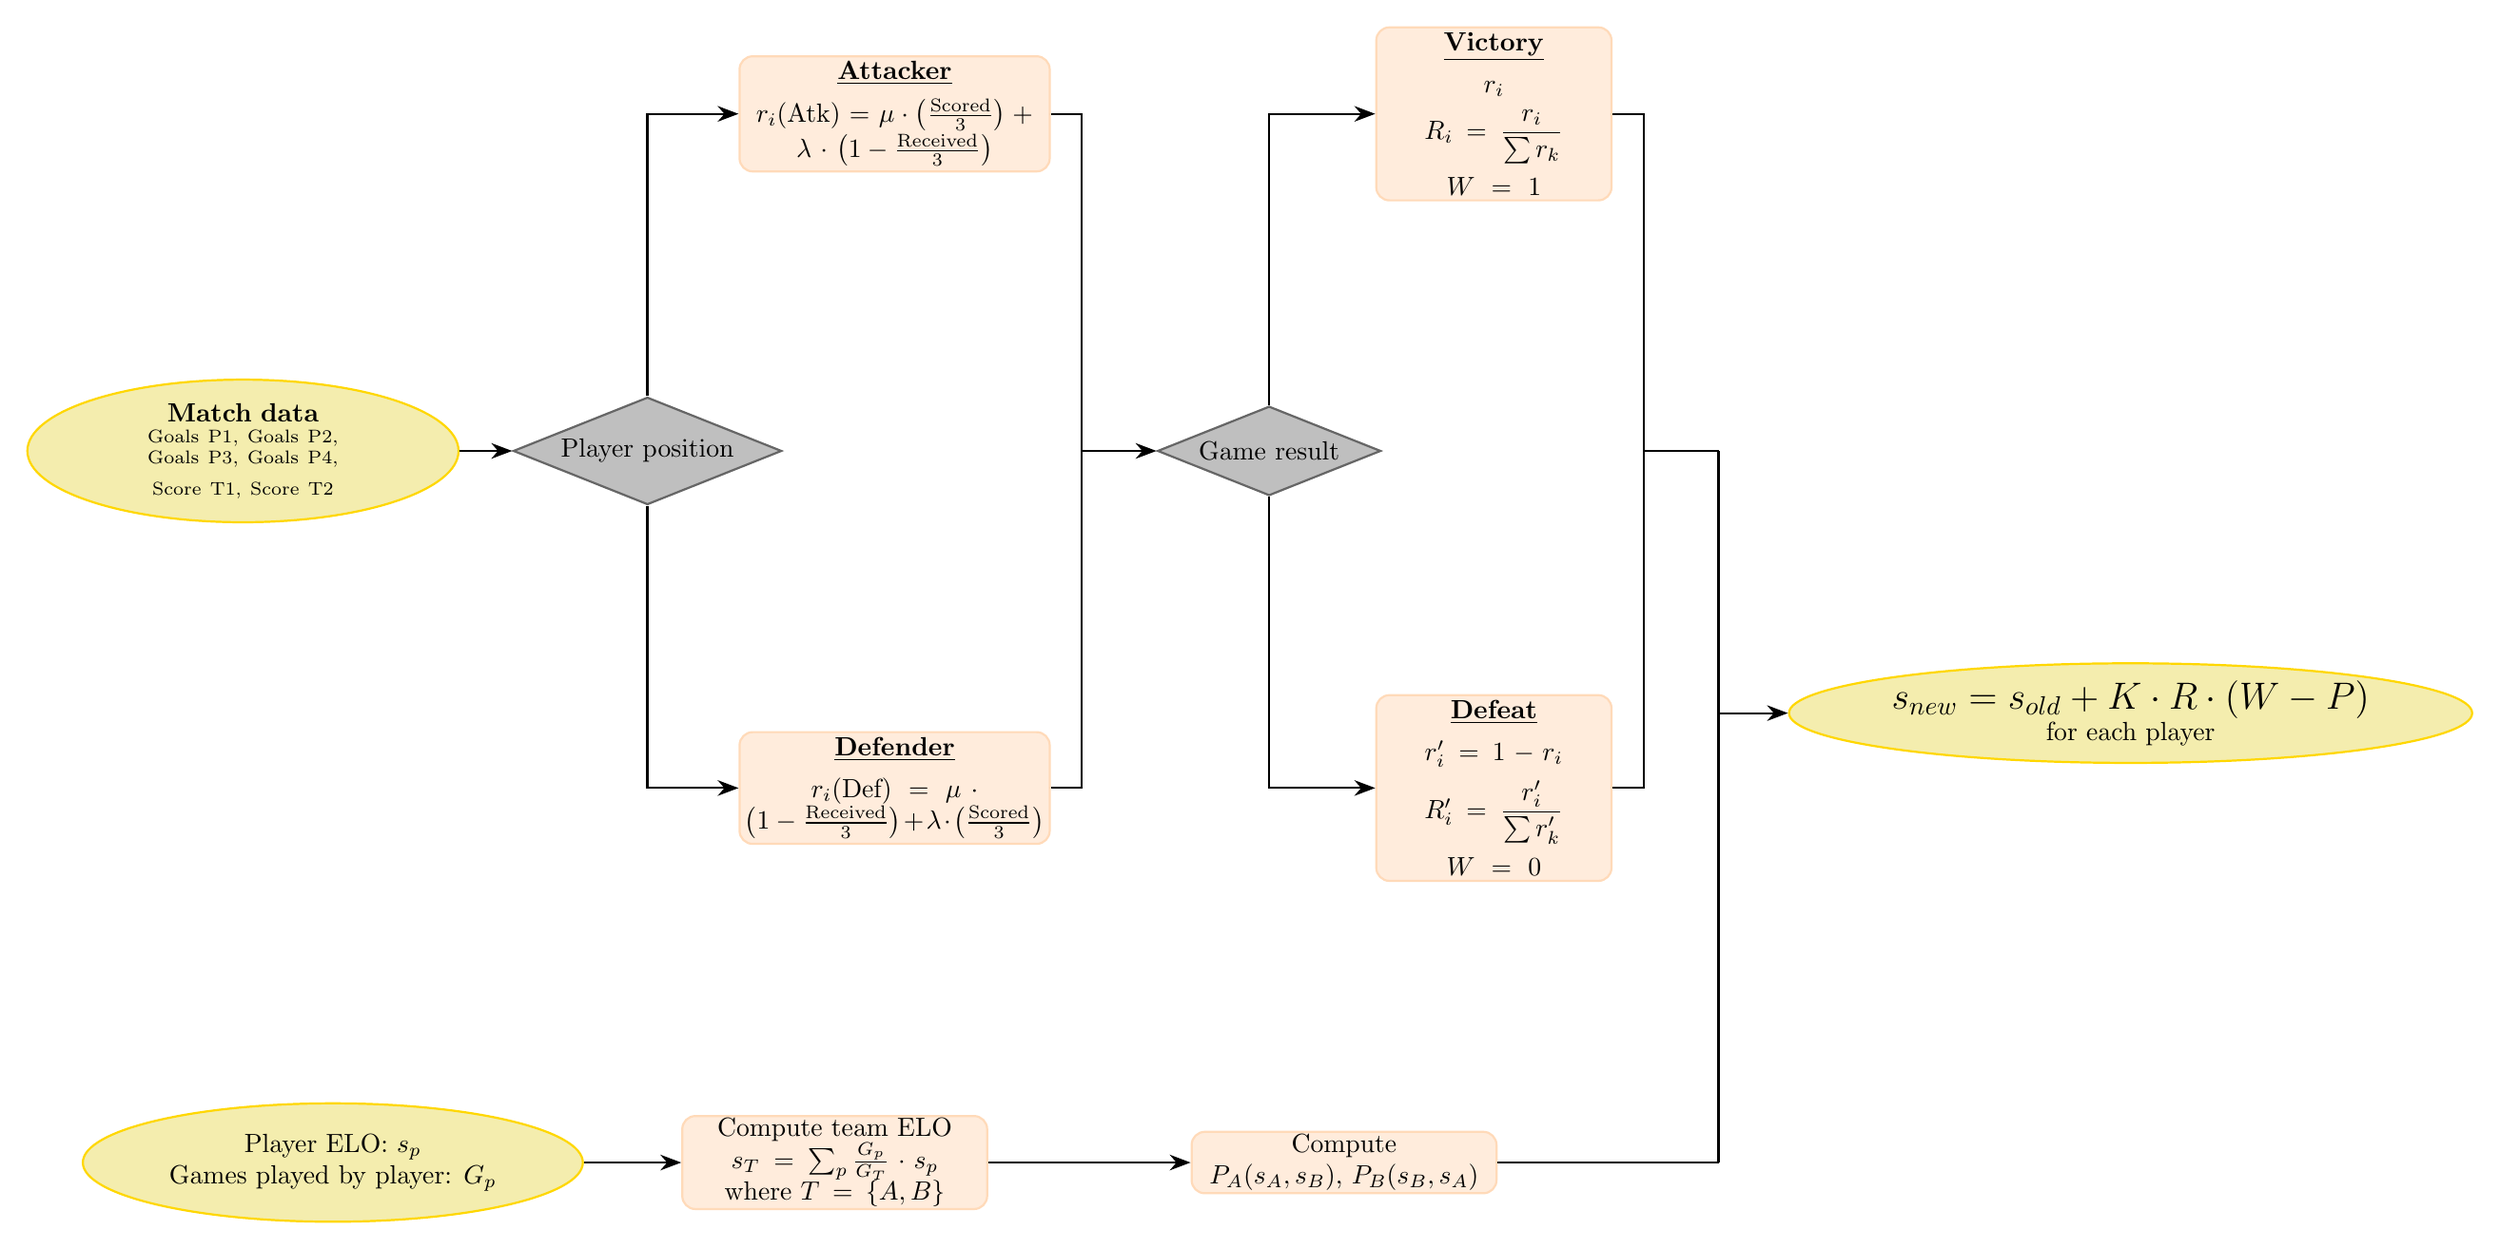
\begin{tikzpicture}[
    myarrow/.style={thick, -{Stealth[scale=1.2]}},
    boxstyle/.style={thick, rounded corners=6pt}
]

    % ==========================================
    % 1. PLAYER PERFORMANCE (Top Branch)
    % ==========================================

    \node[
	    ellipse,
        fill=fillInput,       
        draw=borderInput,          
        thick,              
        rounded corners=5pt,
        inner sep=1pt,     
        text width=4cm,     
        align=center        
    ] (match) at (-1.2, 8) {\textbf{Match data}\\\scriptsize{Goals P1, Goals P2,\\Goals P3, Goals P4,\\Score T1, Score T2}};
   
    \node[diamond, draw, thick, aspect=2.5, inner sep=2pt, fill=fillDecision, draw=borderDecision] (position) at (4.2, 8) {Player position};

     \node[
	    rectangle,
        fill=fillAction,       
        draw=borderAction,          
        thick,              
        rounded corners=5pt,
        inner sep=2pt,     
        text width=4cm,     
        align=center        
    ] (attack) at (7.5, 12.5) {
        \underline{\textbf{Attacker}}\\[4pt]
        $r_i (\text{Atk}) =  \mu \cdot \left(\frac{\text{Scored}}{3} \right) + \lambda \cdot \left( 1- \frac{\text{Received}}{3} \right)$
    };
    
      \node[
	    rectangle,
        fill=fillAction,       
        draw=borderAction,          
        thick,              
        rounded corners=5pt,
        inner sep=2pt,     
        text width=4cm,     
        align=center        
    ] (defend) at (7.5, 3.5) { 
        \underline{\textbf{Defender}}\\[4pt]
        $ r_i (\text{Def}) = \mu \cdot \left( 1 - \frac{\text{Received}}{3} \right) + \lambda \cdot \left( \frac{\text{Scored}}{3} \right)$
    };

    \node[diamond, draw, thick, aspect=2.5, inner sep=2pt, fill=fillDecision, draw=borderDecision] (outcome) at (12.5, 8) {Game result};

    \node[
	    rectangle,
        fill=fillAction,       
        draw=borderAction,          
        thick,              
        rounded corners=5pt,
        inner sep=2pt,     
        text width=3cm,     
        align=center        
    ] (vic) at (15.5, 12.5) {
        \underline{\textbf{Victory}}\\[4pt]
        $r_i$\\[4pt]
        $R_i = \dfrac{r_i}{\sum r_k}$\\[4pt]
        $W=1$
    };

    \node[
	    rectangle,
        fill=fillAction,       
        draw=borderAction,          
        thick,              
        rounded corners=5pt,
        inner sep=2pt,     
        text width=3cm,     
        align=center        
    ] (def) at (15.5, 3.5) {
        \underline{\textbf{Defeat}}\\[4pt]
        $r'_i = 1-r_i$\\[4pt]
        $R'_{i} = \dfrac{r'_i}{\sum r'_k}$\\[4pt]
        $W=0$
    };

    % ==========================================
    % 2. WINNING PROBABILITY (Bottom Branch)
    % ==========================================

    \node[
	    ellipse,
        fill=fillInput,       
        draw=borderInput,          
        thick,              
        inner sep=5pt,     
        align=center        
    ] (sold)  at (0, -1.5) {Player ELO: $s_p$\\Games played by player: $G_p$};

     \node[
	    rectangle,
        fill=fillAction,       
        draw=borderAction,          
        thick,              
        rounded corners=5pt,
        inner sep=1pt,     
        text width=4cm,     
        align=center        
    ] (comp_ELO) at (6.7, -1.5) {Compute team ELO\\ $s_T = \sum_p \frac{G_p}{G_T} \cdot s_p$\\where $T= \{A, B\}$};
    
     \node[
	    rectangle,
        fill=fillAction,       
        draw=borderAction,          
        thick,              
        rounded corners=5pt,
        inner sep=1pt,     
        text width=4cm,     
        align=center        
    ] (comp_pa) at (13.5, -1.5) {Compute\\ $P_A(s_A, s_B)$, $P_B(s_B, s_A)$};
    
    % ==========================================
    % 3. FINAL MERGE (Far Right)
    % ==========================================   
    
    \node[
	    ellipse,
        fill=fillInput,       
        draw=borderInput,          
        thick,              
        rounded corners=5pt,
        inner sep=1pt,     
        align=center        
    ] (final) at (24, 4.5) {\Large $s_{new} = s_{old} + K \cdot R \cdot (W - P)$\\ for each player};


    % ==========================================
    % 4. DRAW CONNECTING ARROWS & LINES (Horizontal Flow)
    % ==========================================
    
    % --- Top Branch Flow ---
    \draw[myarrow] (match) -- (position.west);
    
    % Arrows directly from top and bottom of Player Position diamond
    \draw[myarrow] (position.north) |- (attack.west);
    \draw[myarrow] (position.south) |- (defend.west);
    
    % Merge from Attacker/Defender to Game Result
    \draw[thick] (attack.east) -| (10.0, 8);
    \draw[thick] (defend.east) -| (10.0, 8);
    \draw[myarrow] (10.0, 8) -- (outcome.west);
    
    % Arrows directly from top and bottom of Game Result diamond
    \draw[myarrow] (outcome.north) |- (vic.west);
    \draw[myarrow] (outcome.south) |- (def.west);

    % --- Bottom Branch Flow ---
    \draw[myarrow] (sold) -- (comp_ELO);
    \draw[myarrow] (comp_ELO) -- (comp_pa);

    % --- Final Merge ---
    % Bring Victory/Defeat together at x=18.5
    \draw[thick] (vic.east) -| (17.5, 8);
    \draw[thick] (def.east) -| (17.5, 8);
    \draw[thick] (17.5, 8) -| (18.5, 8);
    
    % Bring Probability calculation to x=18.5
    \draw[thick] (comp_pa.east) -- (18.5, -1.5);
    
    % Connect Top and Bottom branches vertically
    \draw[thick] (18.5, 8) -- (18.5, -1.5);
    
    % Point to Final Update from the vertical junction
    \draw[myarrow] (18.5, 4.5) -- (final.west);

\end{tikzpicture}

\end{document}